\documentclass[letterpaper,9pt,twocolumn,twoside,]{pinp}

%% Some pieces required from the pandoc template
\providecommand{\tightlist}{%
  \setlength{\itemsep}{0pt}\setlength{\parskip}{0pt}}

% Use the lineno option to display guide line numbers if required.
% Note that the use of elements such as single-column equations
% may affect the guide line number alignment.

\usepackage[T1]{fontenc}
\usepackage[utf8]{inputenc}

% pinp change: the geometry package layout settings need to be set here, not in pinp.cls
\geometry{layoutsize={0.95588\paperwidth,0.98864\paperheight},%
  layouthoffset=0.02206\paperwidth, layoutvoffset=0.00568\paperheight}

\definecolor{pinpblue}{HTML}{185FAF}  % imagecolorpicker on blue for new R logo
\definecolor{pnasbluetext}{RGB}{101,0,0} %



\title{Linear regression model for predicting percent body fat}

\author[]{First Author}


\setcounter{secnumdepth}{0}

% Please give the surname of the lead author for the running footer
\leadauthor{}

% Keywords are not mandatory, but authors are strongly encouraged to provide them. If provided, please include two to five keywords, separated by the pipe symbol, e.g:
 

\begin{abstract}
Per cent body fat, although an accurate health indicator, is difficult
and costly to measure. We ran a series of multiple regression analyses
with the aim of creating a model to accurately estimate a male's
percentage of body fat from a few easily obtained body measurements. Our
final model was selected using the backwards stepwise method, with BIC
as our threshold indicator. The model contains the predictor variables:
age, height, abdomen and wrist circumference.
\end{abstract}

\dates{This version was compiled on \today} 


% initially we use doi so keep for backwards compatibility
% new name is doi_footer

\pinpfootercontents{YourPackage Vignette}

\begin{document}

% Optional adjustment to line up main text (after abstract) of first page with line numbers, when using both lineno and twocolumn options.
% You should only change this length when you've finalised the article contents.
\verticaladjustment{-2pt}

\maketitle
\thispagestyle{firststyle}
\ifthenelse{\boolean{shortarticle}}{\ifthenelse{\boolean{singlecolumn}}{\abscontentformatted}{\abscontent}}{}

% If your first paragraph (i.e. with the \dropcap) contains a list environment (quote, quotation, theorem, definition, enumerate, itemize...), the line after the list may have some extra indentation. If this is the case, add \parshape=0 to the end of the list environment.

\acknow{This template package builds upon, and extends, the work of the
excellent gratefully acknowledged as this work would not have been
possible without them. Our extensions are under the same respective
licensing term
\href{https://cran.r-project.org/package=rticles}{rticles} package, and
both packages rely on the
\href{http://www.pnas.org/site/authors/latex.xhtml}{PNAS LaTeX} macros.
Both these sources are
(\href{https://www.gnu.org/licenses/gpl-3.0.en.html}{GPL-3} and
\href{https://www.latex-project.org/lppl/}{LPPL (\textgreater= 1.3)}).}

\hypertarget{introduction}{%
\subsection{Introduction}\label{introduction}}

Obesity has become an increasingly important global health problem
(Jaacks et al., 2019). It is defined as the accumulation of excess fat
in the body, to the extent of impacting an individual's health and
well-being (Deurenberg \& Yap, 1999). Body fat percentage is a
measurement that can help define individuals into a weight category,
such as obese (Trung et al., 2019). Furthermore, body fat percentage can
be used as a heath and fitness indicator. However, measuring body fat
percentage is costly and difficult to accurately measure (Deurenberg et
al., 2002). Hence, the aim of our analysis is to create a model that
estimates a male's body fat percentage from easily accessible
measurements.

\hypertarget{data-set}{%
\subsection{Data Set}\label{data-set}}

Our data set contains the measurements of 250 men of various ages
(Bodyfat DASL, 2022). The per cent body fat of each male was estimated
from their body density (Penrose et al., 1985). In addition, measures
such as age, height, weight, and the circumference of the neck, abdomen
and chest were taken. In total there are 15 measurements, all classified
as continuous, apart from age which is discrete. For data cleaning, we
removed the density variable and two observations with less than one per
cent body fat. In terms of data wrangling we converted the units for
height and weight into the metric system and calculated BMI for the
remaining 248 observations.

\hypertarget{model-selection}{%
\subsection{Model selection}\label{model-selection}}

For our model selection process we considered both backwards and
forwards stepwise selection. We decided to go with the backwards
process, as our research indicated backwards models were generally
better equipped to deal with collinearity. Because a backwards process
considers the full set of variables initially, it is more likely to keep
a set of collinear variables whereas a forwards model is more likely to
not include any of the correlated variables. Because our data set
included a range of physical measurements which are all correlated to
some extent, we felt we therefore needed to use a backwards stepwise
selection process.

Noting the high p value of the intercept in our models, we generated
models without intercepts and found the adjusted R squared values of
those models to be significantly higher (see figure 1). We therefore
decided to remove the intercepts from all future models.

BMI is often used as an indicator of healthy weight adjusted for height,
we calculated BMI for the sample and generated a model which used BMI as
a composite for height and weight. The fit of both models was very
comparable (see figure 2), with nearly identical adjusted R squared and
AIC values. We decided to move forward with the original variable
specification because the BMI model used more variables overall. Given
that the models had very similar fit we chose the simpler model both for
the practical applicability of the model and because we believed the BMI
model would perform worse in out of sample testing due to possible
over-fitting.

The two standard criterion for automated model selection are AIC and BIC
(Bayesian Information Criterion). We decided to examine models using
both criterion (see figure 3). The models had identical adjusted R
squared, with the BIC model using two fewer variables. We decided to
examine both models using out of sample performance evaluation methods.

\hypertarget{performance}{%
\subsection{Performance:}\label{performance}}

To evaluate the performance of our AIC and BIC models we used 10 fold
cross validation

\hypertarget{assumption-checking}{%
\subsection{Assumption Checking}\label{assumption-checking}}

\begin{itemize}
\tightlist
\item
  \textbf{Linearity:} By looking at the plot of the residuals against
  the fitted values (Figure \textbackslash4), we can see a fairly
  horizontal line to 0 however it's a little worrying near the end
  portion on the line where it seems to develop a sort of declining
  pattern. This inspired a further look into the assumption through
  looking at each predictor variable plotted against body fat percentage
  individually (Figure \textbackslash5) which seems to demonstrate
  linearity as points above and below the line are fairly equal in
  proportion.
\item
  \textbf{Independence:} Independence can't really be tested through the
  data, we just placed trust in the fact that the data was collected
  independently of each other allowing errors to be independent. This
  assumption should be satisfied at the data comes from the Brigham
  Young University which is a fairly trusted source, they state the data
  comes from 250 men at varying ages hopefully indicating independence.
\item
  \textbf{Normality:} In the normality assumption we are assuming the
  residual error is normally distributed. Judging from the qq-plot
  generated from the residuals (Figure \textbackslash4), it seems to
  follow the line fairly well up until the end portion, which again was
  a little worrying. However even if qq-plot doesn't demonstrate
  normality we should be able to argue the Central Limit Theorem
  allowing for this assumption due to the large number of observations.
\item
  \textbf{Homoscedasticity:} Through plotting the standardized residuals
  and fitted values (Figure \textbackslash4) we should be able to test
  for homoscedasticity where residuals are assumed to have a constant
  variance. In order to have this assumption the points should be
  equally spread above and below the line as well as having a line
  horizontal (or void of any patterns). The graph shows equally spread
  points and the line isn't horizontal though it seems void of patterns
  enough to be able to assume homoscedasticity.
\end{itemize}

\hypertarget{results}{%
\subsection{Results}\label{results}}

Our final model is obtained from a backward stepwise linear regression
model with BIC as selection criteria. This is the best fit among all our
models with only 4 predictors.

\hypertarget{discussion}{%
\subsection{Discussion}\label{discussion}}

\begin{itemize}
\item
  Effectiveness Model: Body\_Fat\_Percentage = 0.05795 * Age - 11.27374
  * Height + 0.76046 * Abdomen - 1.84242 * Wrist Our model has a total
  of four variables, each of which has a p-value less than 0.05. This
  represents a significant effect of each of the variables on the
  model.Our adjusted R square value is 0.9586.This represents that our
  model has a high predictive accuracy. Our model can be used by back
  health organizations to measure the healthiness of people's body fat
  percentage.
\item
  Limitation 1.We used only physical data as a reference. This leads to
  a large error when dealing with special populations. For example, fit
  elderly people, people who are short in height but work out regularly
  and people of different races.. Future study to overcome
  limitations:We consider increasing the number of elements including
  daily calorie intake, time spent in daily exercise, etc. to reduce the
  effect of single body data on body fat percentage.
\end{itemize}

\hypertarget{conclusion}{%
\subsection{Conclusion}\label{conclusion}}

TBC

\hypertarget{appendix}{%
\subsection{Appendix}\label{appendix}}

Figure 1 (Testing the intercept):

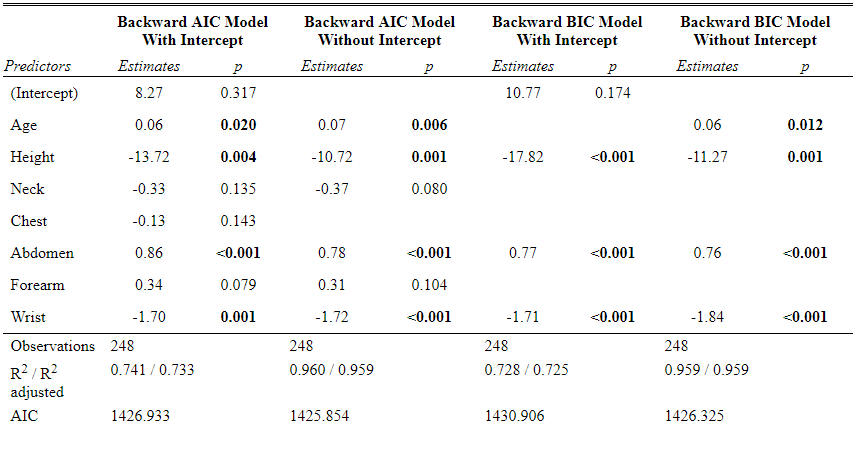
\includegraphics{images/intercepttest.png} Figure 2 (BMI Specification):

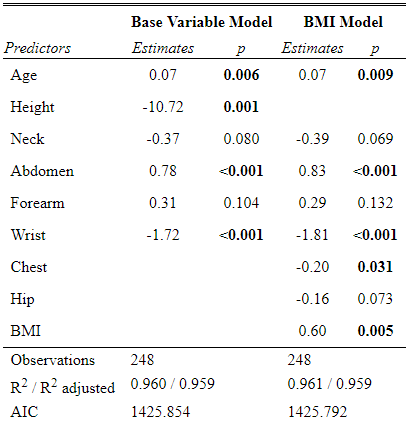
\includegraphics{BMItest.png}

Figure 3 (AIC vs BIC):

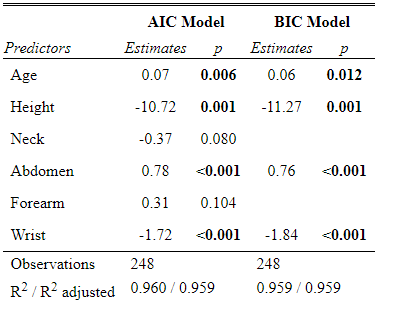
\includegraphics{AIC vs BIC.png} Figure 4 (Assumptions Graphs)
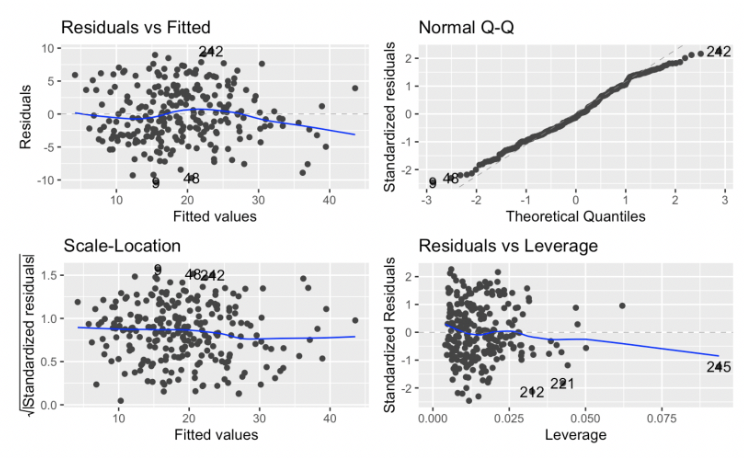
\includegraphics{Assumptions.png} Figure 5 (Linearity further explored)
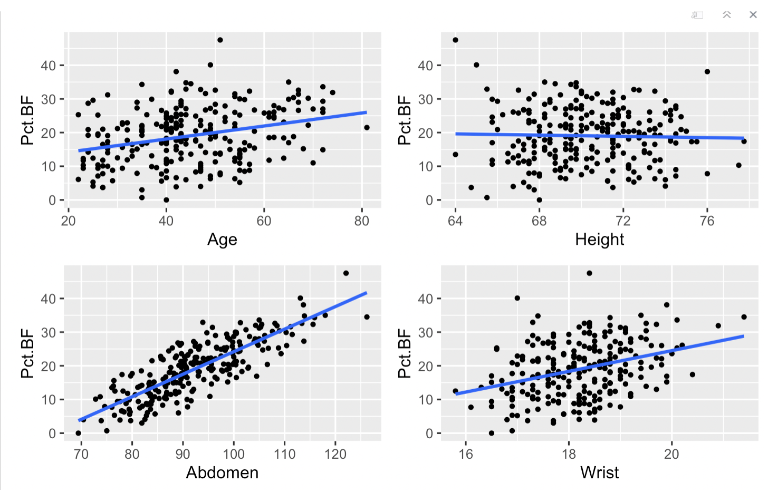
\includegraphics{Linearitytest.png}

\hypertarget{references}{%
\subsection{References:}\label{references}}

Bodyfat Data and Story Library (DASL). (2022).
\url{https://dasl.datadescription.com/datafile/bodyfat/}

Deurenberg, P., \& Yap, M. (1999). The assessment of obesity: methods
for measuring body fat and global prevalence of obesity. Best practice
\& research clinical endocrinology \& metabolism, 13(1), 1-11.
\url{https://doi.org/10.1053/beem.1999.0003}

Deurenberg, P., Yap, M., \& Guricci, S. (2002). Asians are different
from Caucasians and from each other in their body mass index/body fat
per cent relationship. Obesity reviews, 3(3), 141-146.
\url{https://doi.org/10.1046/j.1467-789X.2002.00065.x}

Jaacks, L. M., Vandevijvere, S., Pan, A., McGowan, C. J., Wallace, C.,
Imamura, F., Mozaffarian D., Swinburn, B \& Ezzati, M. (2019). The
obesity transition: stages of the global epidemic. The Lancet Diabetes
\& Endocrinology, 7(3), 231-240.
\url{https://doi.org/10.1016/S2213-8587(19)30026-9}

Penrose, K. W., Nelson, A. G., \& Fisher, A. G. (1985). Generalized body
composition prediction equation for men using simple measurement
techniques. Medicine \& Science in Sports \& Exercise, 17(2), 189.
\url{DOI:10.1249/00005768-198504000-00037}

Trung, N. N., Chu, D. T., \& Hanh, N. T. H. (2019). Percentage body fat
is as a good indicator for determining adolescents who are overweight or
obese: a cross-sectional study in Vietnam. Osong public health and
research perspectives, 10(2), 108. DOI: 10.24171/j.phrp.2019.10.2.10

%\showmatmethods
\showacknow


\bibliography{pinp}
\bibliographystyle{jss}



\end{document}
